
% Section headings appear in the Table of contents
\section[Basic structuring]{Basic structuring: columns, relative sizes}
\begin{frame}{Structuring} 
  In the motivation section we have already seen how to
  use 
  \begin{itemize}
  \item paragraphs
  \item itemi[z]ation and
  \item uncover
  \end{itemize}
  to structure our frames [slides].

  \vfill
  \uncover<2->{There are a few other useful elements}
\end{frame}

\begin{frame}{Columns}
\parbox{\textwidth}{
  A nice and easy option to present information in columns with
  minimal work (certainly easier than using \ltx{minipage}) is
  to use columns:}

  \vfill

  \begin{columns}
    \begin{column}{.51\textwidth}
      \uncover<2->{Some text can go here and fill this
        column.

        Text will be formatted same as a full page.
        }      
    \end{column}
    \begin{column}{.4\textwidth}
      \uncover<3->{And some text can go here and fill this
        column.}
      \uncover<4->{
        Easy. 
        }
    \end{column}
  \end{columns}

\vfill
\uncover<5->{
I have used the \ltx{textwidth} variable to control the width of the columns.
You need to leave a bit of space between each columns, 0.09\ltx{textwidth} works
fine, so the width of my two columns sums to 0.91\ltx{textwidth}

\vfill
Note also the use of \ltx{vfill} to provide vertical rubber space
and help Latex to space the blocks out vertically on the frame.
}
\end{frame}


\section[Figures]{How to align and uncover figures}

\begin{frame}{How to (and how not to) include figures}
  Don't use the {\tt figure} environment in slides. {\tt figure}
  creates a ``floating body'' that Latex can place where best suited, 
  including the number and caption. Not what you want here. Use
  a straight \ltx{includegraphics}, and \ltx{centerline}
  to centre.

  \uncover<2-> {
  \ltx{includegraphics} can also be ``uncovered'', but if you
  want to reserve the space for the figure, i.e.~not have any
  preceding text move when the figure is shown, then you have
  to do a bit of extra work as in this example.
  }

  \invisible<1-2>{
    \centerline{
       \includegraphics<1-2>[width=.6\textwidth]{aflo-header}}         }
  \centerline{\includegraphics<3->[width=.6\textwidth]{aflo-header}}

  \uncover<4->{Remove the \ltx{invisible} image to see what happens
    without. You can see even with the phantom image, when you
    remove a bit of text, there is still a
    bit of a wobble, duckDuckGo is your friend to try
    other solutions.}
  
\end{frame}

\begin{frame}{Lining up figures in rows and columns}

You can either use the \ltx{tabular} environment and include
each figure in a box of the table, or simply line up with 
appropriate spacing. 

\vfill
Note that for Latex a graphic is just a
box, same as a letter, and will be lined up as a letter.

\vfill
%\begin{figure}
\hfil
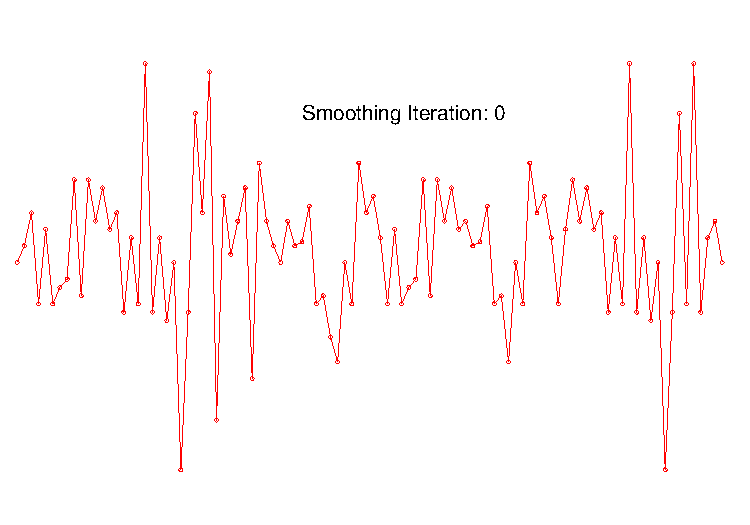
\includegraphics[width=.17\textwidth]{figures/animations/LaplacianSmoothing/smoothingEx-1}\hfil
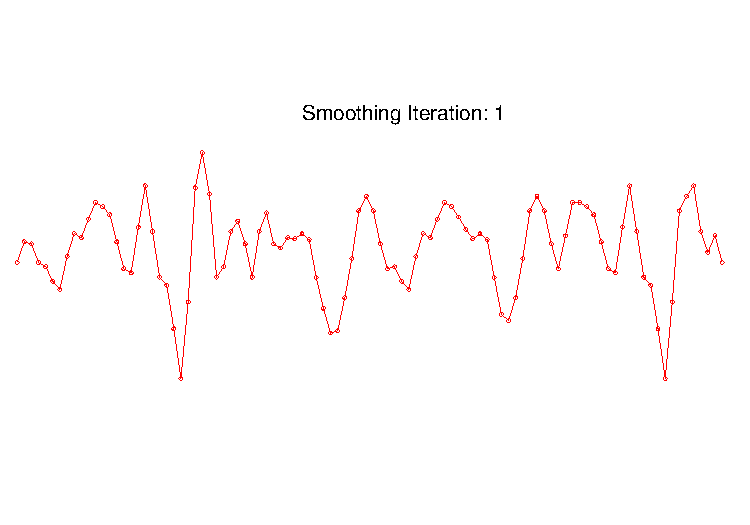
\includegraphics[width=.17\textwidth]{figures/animations/LaplacianSmoothing/smoothingEx-2}\hfil
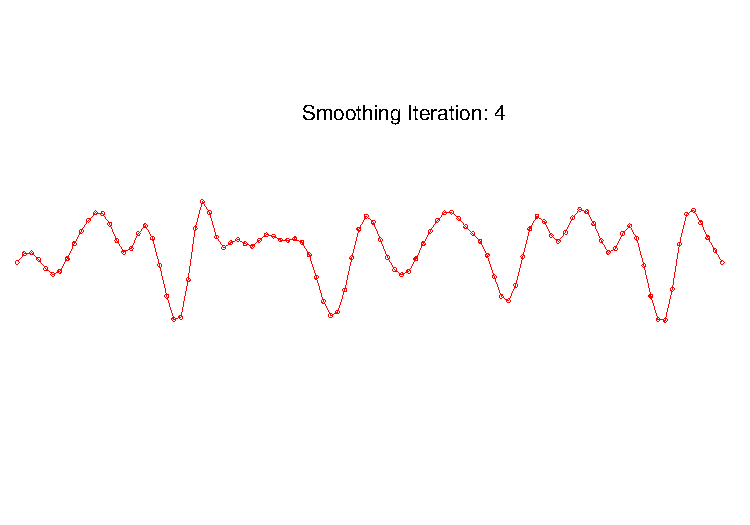
\includegraphics[width=.17\textwidth]{figures/animations/LaplacianSmoothing/smoothingEx-5}\hfil
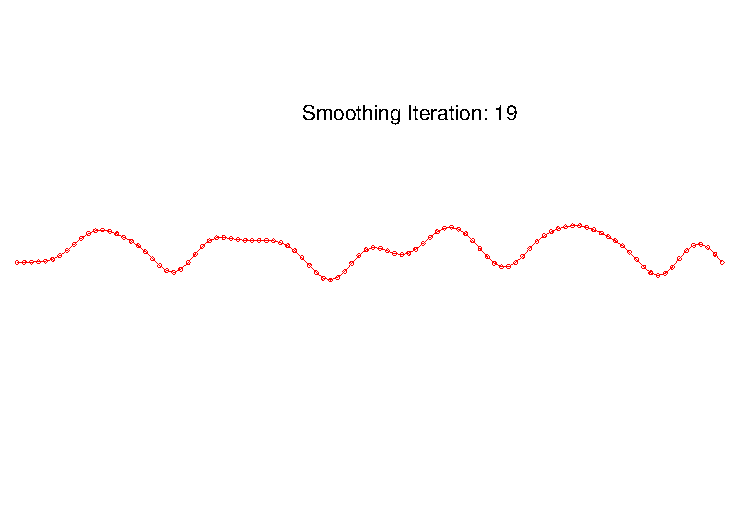
\includegraphics[width=.17\textwidth]{figures/animations/LaplacianSmoothing/smoothingEx-20}\hfil
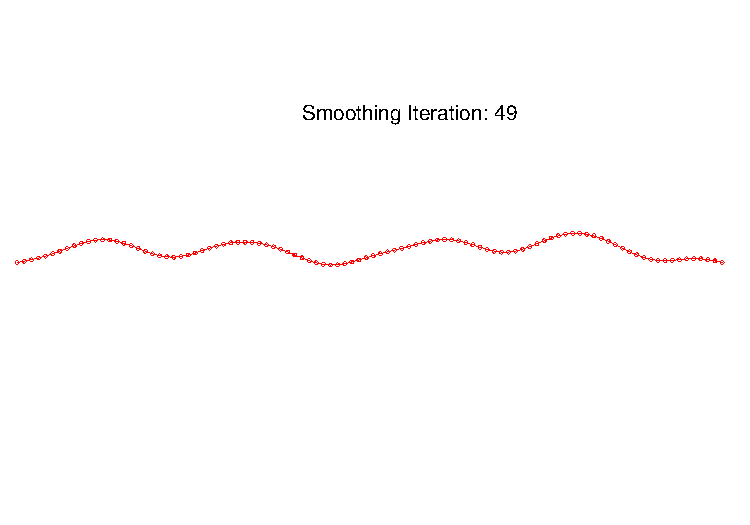
\includegraphics[width=.17\textwidth]{figures/animations/LaplacianSmoothing/smoothingEx-50}\hfil
%\end{figure}

%\smallskip

\hfil
\parbox{.17\textwidth}{\centerline{Iter 1  }}\hfil
\parbox{.17\textwidth}{\centerline{Iter 2  }}\hfil
\parbox{.17\textwidth}{\centerline{Iter 5  }}\hfil
\parbox{.17\textwidth}{\centerline{Iter 20 }}\hfil
\parbox{.17\textwidth}{\centerline{Iter 50 }}\hfil

\vfill
\uncover<2->{
Note the extensive use of relative measurements for figure scaling,
such as .17\ltx{textwidth}, rather than absolute measurements. This
also makes it easy to keep scalings when moving blocks of figures
between the paper and the talk.
}

\end{frame}


\begin{frame}{A neat and clean way to include graphics}
  \begin{itemize}
  \item Many tools (gnuplot, Inkscape, xfig) support output of Latex graphics
  \item Advantage: Full support of Latex typesetting, formulae etc.
  \item Text looks clean and has the right size. No more figures with unreadable text (Well, within a certain range of scaling).
  \item Image size can be changed without changing text size
  \item Gnuplot: use \texttt{set terminal epslatex size 10cm,7cm color; set output "example.eps"}
  \item Then run \texttt{epstopdf fd.eps} in terminal to create pdf image if you are using pdflatex
  \end{itemize}

\slidefoot{Contributed by JH}
\
\end{frame}


\begin{frame}{Example graphic produced with gnuplot}
  \begin{center}
    % GNUPLOT: LaTeX picture with Postscript
\begingroup
  \makeatletter
  \providecommand\color[2][]{%
    \GenericError{(gnuplot) \space\space\space\@spaces}{%
      Package color not loaded in conjunction with
      terminal option `colourtext'%
    }{See the gnuplot documentation for explanation.%
    }{Either use 'blacktext' in gnuplot or load the package
      color.sty in LaTeX.}%
    \renewcommand\color[2][]{}%
  }%
  \providecommand\includegraphics[2][]{%
    \GenericError{(gnuplot) \space\space\space\@spaces}{%
      Package graphicx or graphics not loaded%
    }{See the gnuplot documentation for explanation.%
    }{The gnuplot epslatex terminal needs graphicx.sty or graphics.sty.}%
    \renewcommand\includegraphics[2][]{}%
  }%
  \providecommand\rotatebox[2]{#2}%
  \@ifundefined{ifGPcolor}{%
    \newif\ifGPcolor
    \GPcolortrue
  }{}%
  \@ifundefined{ifGPblacktext}{%
    \newif\ifGPblacktext
    \GPblacktextfalse
  }{}%
  % define a \g@addto@macro without @ in the name:
  \let\gplgaddtomacro\g@addto@macro
  % define empty templates for all commands taking text:
  \gdef\gplbacktext{}%
  \gdef\gplfronttext{}%
  \makeatother
  \ifGPblacktext
    % no textcolor at all
    \def\colorrgb#1{}%
    \def\colorgray#1{}%
  \else
    % gray or color?
    \ifGPcolor
      \def\colorrgb#1{\color[rgb]{#1}}%
      \def\colorgray#1{\color[gray]{#1}}%
      \expandafter\def\csname LTw\endcsname{\color{white}}%
      \expandafter\def\csname LTb\endcsname{\color{black}}%
      \expandafter\def\csname LTa\endcsname{\color{black}}%
      \expandafter\def\csname LT0\endcsname{\color[rgb]{1,0,0}}%
      \expandafter\def\csname LT1\endcsname{\color[rgb]{0,1,0}}%
      \expandafter\def\csname LT2\endcsname{\color[rgb]{0,0,1}}%
      \expandafter\def\csname LT3\endcsname{\color[rgb]{1,0,1}}%
      \expandafter\def\csname LT4\endcsname{\color[rgb]{0,1,1}}%
      \expandafter\def\csname LT5\endcsname{\color[rgb]{1,1,0}}%
      \expandafter\def\csname LT6\endcsname{\color[rgb]{0,0,0}}%
      \expandafter\def\csname LT7\endcsname{\color[rgb]{1,0.3,0}}%
      \expandafter\def\csname LT8\endcsname{\color[rgb]{0.5,0.5,0.5}}%
    \else
      % gray
      \def\colorrgb#1{\color{black}}%
      \def\colorgray#1{\color[gray]{#1}}%
      \expandafter\def\csname LTw\endcsname{\color{white}}%
      \expandafter\def\csname LTb\endcsname{\color{black}}%
      \expandafter\def\csname LTa\endcsname{\color{black}}%
      \expandafter\def\csname LT0\endcsname{\color{black}}%
      \expandafter\def\csname LT1\endcsname{\color{black}}%
      \expandafter\def\csname LT2\endcsname{\color{black}}%
      \expandafter\def\csname LT3\endcsname{\color{black}}%
      \expandafter\def\csname LT4\endcsname{\color{black}}%
      \expandafter\def\csname LT5\endcsname{\color{black}}%
      \expandafter\def\csname LT6\endcsname{\color{black}}%
      \expandafter\def\csname LT7\endcsname{\color{black}}%
      \expandafter\def\csname LT8\endcsname{\color{black}}%
    \fi
  \fi
  \setlength{\unitlength}{0.0500bp}%
  \begin{picture}(5668.00,3968.00)%
    \gplgaddtomacro\gplbacktext{%
      \csname LTb\endcsname%
      \put(718,704){\makebox(0,0)[r]{\strut{}\scriptsize $10^{-10}$}}%
      \put(718,1030){\makebox(0,0)[r]{\strut{}\scriptsize $10^{-9}$}}%
      \put(718,1355){\makebox(0,0)[r]{\strut{}\scriptsize $10^{-8}$}}%
      \put(718,1681){\makebox(0,0)[r]{\strut{}\scriptsize $10^{-7}$}}%
      \put(718,2006){\makebox(0,0)[r]{\strut{}\scriptsize $10^{-6}$}}%
      \put(718,2332){\makebox(0,0)[r]{\strut{}\scriptsize $10^{-5}$}}%
      \put(718,2657){\makebox(0,0)[r]{\strut{}\scriptsize $10^{-4}$}}%
      \put(718,2983){\makebox(0,0)[r]{\strut{}\scriptsize $10^{-3}$}}%
      \put(718,3308){\makebox(0,0)[r]{\strut{}\scriptsize $10^{-2}$}}%
      \put(850,484){\makebox(0,0){\strut{}\scriptsize $10^{-12}$}}%
      \put(1726,484){\makebox(0,0){\strut{}\scriptsize $10^{-10}$}}%
      \put(2602,484){\makebox(0,0){\strut{}\scriptsize $10^{-8}$}}%
      \put(3478,484){\makebox(0,0){\strut{}\scriptsize $10^{-6}$}}%
      \put(4354,484){\makebox(0,0){\strut{}\scriptsize $10^{-4}$}}%
      \put(5230,484){\makebox(0,0){\strut{}\scriptsize $10^{-2}$}}%
      \put(80,2006){\rotatebox{90}{\makebox(0,0){\strut{}error}}}%
      \put(3259,154){\makebox(0,0){\strut{}Finite difference perturbation}}%
      \put(3259,3638){\makebox(0,0){\strut{}Validation of adjoint gradient wrt. finite differences}}%
    }%
    \gplgaddtomacro\gplfronttext{%
      \csname LTb\endcsname%
      \put(4945,3157){\makebox(0,0)[r]{\strut{}\scriptsize $\Vert\nabla_{FD}-\nabla_{adj}\Vert_2$}}%
    }%
    \gplbacktext
    \put(0,0){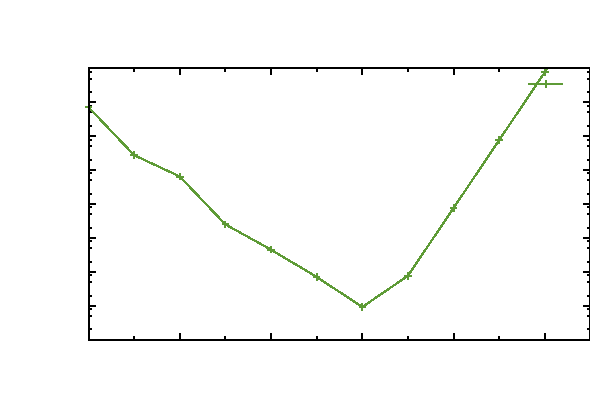
\includegraphics{fdvalidation}}%
    \gplfronttext
  \end{picture}%
\endgroup
    
  \end{center}
\end{frame}



\begin{frame}{And half the size}
  Some scaling can be done without re-running
  gnuplot by modifying the \ltx{setlength} statement in the 
  text part of the figure to an appropriate fraction, and then 
  adding a [scale=] optional argument to the \ltx{includegraphics}
  command. See the example in {\tt fdvalidation\_half.tex}.

  \begin{center}
    % GNUPLOT: LaTeX picture with Postscript
\begingroup
  \makeatletter
  \providecommand\color[2][]{%
    \GenericError{(gnuplot) \space\space\space\@spaces}{%
      Package color not loaded in conjunction with
      terminal option `colourtext'%
    }{See the gnuplot documentation for explanation.%
    }{Either use 'blacktext' in gnuplot or load the package
      color.sty in LaTeX.}%
    \renewcommand\color[2][]{}%
  }%
  \providecommand\includegraphics[2][]{%
    \GenericError{(gnuplot) \space\space\space\@spaces}{%
      Package graphicx or graphics not loaded%
    }{See the gnuplot documentation for explanation.%
    }{The gnuplot epslatex terminal needs graphicx.sty or graphics.sty.}%
    \renewcommand\includegraphics[2][]{}%
  }%
  \providecommand\rotatebox[2]{#2}%
  \@ifundefined{ifGPcolor}{%
    \newif\ifGPcolor
    \GPcolortrue
  }{}%
  \@ifundefined{ifGPblacktext}{%
    \newif\ifGPblacktext
    \GPblacktextfalse
  }{}%
  % define a \g@addto@macro without @ in the name:
  \let\gplgaddtomacro\g@addto@macro
  % define empty templates for all commands taking text:
  \gdef\gplbacktext{}%
  \gdef\gplfronttext{}%
  \makeatother
  \ifGPblacktext
    % no textcolor at all
    \def\colorrgb#1{}%
    \def\colorgray#1{}%
  \else
    % gray or color?
    \ifGPcolor
      \def\colorrgb#1{\color[rgb]{#1}}%
      \def\colorgray#1{\color[gray]{#1}}%
      \expandafter\def\csname LTw\endcsname{\color{white}}%
      \expandafter\def\csname LTb\endcsname{\color{black}}%
      \expandafter\def\csname LTa\endcsname{\color{black}}%
      \expandafter\def\csname LT0\endcsname{\color[rgb]{1,0,0}}%
      \expandafter\def\csname LT1\endcsname{\color[rgb]{0,1,0}}%
      \expandafter\def\csname LT2\endcsname{\color[rgb]{0,0,1}}%
      \expandafter\def\csname LT3\endcsname{\color[rgb]{1,0,1}}%
      \expandafter\def\csname LT4\endcsname{\color[rgb]{0,1,1}}%
      \expandafter\def\csname LT5\endcsname{\color[rgb]{1,1,0}}%
      \expandafter\def\csname LT6\endcsname{\color[rgb]{0,0,0}}%
      \expandafter\def\csname LT7\endcsname{\color[rgb]{1,0.3,0}}%
      \expandafter\def\csname LT8\endcsname{\color[rgb]{0.5,0.5,0.5}}%
    \else
      % gray
      \def\colorrgb#1{\color{black}}%
      \def\colorgray#1{\color[gray]{#1}}%
      \expandafter\def\csname LTw\endcsname{\color{white}}%
      \expandafter\def\csname LTb\endcsname{\color{black}}%
      \expandafter\def\csname LTa\endcsname{\color{black}}%
      \expandafter\def\csname LT0\endcsname{\color{black}}%
      \expandafter\def\csname LT1\endcsname{\color{black}}%
      \expandafter\def\csname LT2\endcsname{\color{black}}%
      \expandafter\def\csname LT3\endcsname{\color{black}}%
      \expandafter\def\csname LT4\endcsname{\color{black}}%
      \expandafter\def\csname LT5\endcsname{\color{black}}%
      \expandafter\def\csname LT6\endcsname{\color{black}}%
      \expandafter\def\csname LT7\endcsname{\color{black}}%
      \expandafter\def\csname LT8\endcsname{\color{black}}%
    \fi
  \fi
%  Original size:
%  \setlength{\unitlength}{0.0500bp}%
% Half the original size
  \setlength{\unitlength}{0.0250bp}%
  \begin{picture}(5668.00,3968.00)%
    \gplgaddtomacro\gplbacktext{%
      \csname LTb\endcsname%
      \put(718,704){\makebox(0,0)[r]{\strut{}\scriptsize $10^{-10}$}}%
      \put(718,1030){\makebox(0,0)[r]{\strut{}\scriptsize $10^{-9}$}}%
      \put(718,1355){\makebox(0,0)[r]{\strut{}\scriptsize $10^{-8}$}}%
      \put(718,1681){\makebox(0,0)[r]{\strut{}\scriptsize $10^{-7}$}}%
      \put(718,2006){\makebox(0,0)[r]{\strut{}\scriptsize $10^{-6}$}}%
      \put(718,2332){\makebox(0,0)[r]{\strut{}\scriptsize $10^{-5}$}}%
      \put(718,2657){\makebox(0,0)[r]{\strut{}\scriptsize $10^{-4}$}}%
      \put(718,2983){\makebox(0,0)[r]{\strut{}\scriptsize $10^{-3}$}}%
      \put(718,3308){\makebox(0,0)[r]{\strut{}\scriptsize $10^{-2}$}}%
      \put(850,484){\makebox(0,0){\strut{}\scriptsize $10^{-12}$}}%
      \put(1726,484){\makebox(0,0){\strut{}\scriptsize $10^{-10}$}}%
      \put(2602,484){\makebox(0,0){\strut{}\scriptsize $10^{-8}$}}%
      \put(3478,484){\makebox(0,0){\strut{}\scriptsize $10^{-6}$}}%
      \put(4354,484){\makebox(0,0){\strut{}\scriptsize $10^{-4}$}}%
      \put(5230,484){\makebox(0,0){\strut{}\scriptsize $10^{-2}$}}%
      \put(80,2006){\rotatebox{90}{\makebox(0,0){\strut{}error}}}%
      \put(3259,154){\makebox(0,0){\strut{}Finite difference perturbation}}%
      \put(3259,3638){\makebox(0,0){\strut{}Validation of adjoint gradient wrt. finite differences}}%
    }%
    \gplgaddtomacro\gplfronttext{%
      \csname LTb\endcsname%
      \put(4945,3157){\makebox(0,0)[r]{\strut{}\scriptsize $\Vert\nabla_{FD}-\nabla_{adj}\Vert_2$}}%
    }%
    \gplbacktext
%   Original include, unscaled.
%    \put(0,0){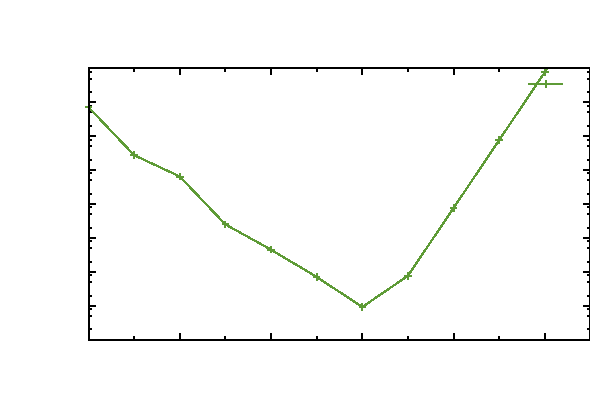
\includegraphics{fdvalidation}}%
%   Scaled-down include
    \put(0,0){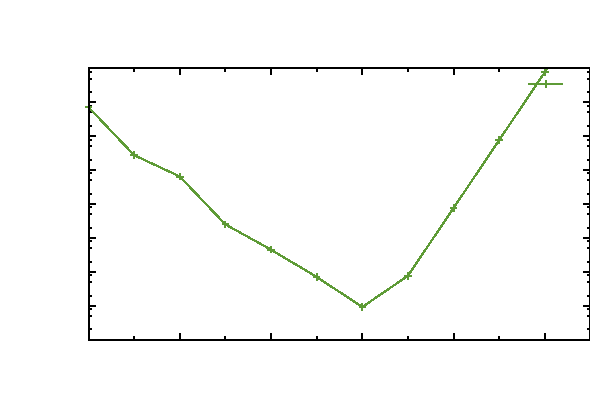
\includegraphics[scale=.5]{fdvalidation}}%
    \gplfronttext
  \end{picture}%
\endgroup
    
  \end{center}

  \uncover<2->{You can see that there are limits to scaling. But
   $\pm20\%$ is often ok.}
\end{frame}



\begin{frame}{Overlays}
 
  If you want to show different parts using the same space,
  then you can 'reserve' that space with \ltx{overlayarea}:

  \vfill

  \begin{overlayarea}{\textwidth}{.5\textheight}
    \only<1>{\centerline{% GNUPLOT: LaTeX picture with Postscript
\begingroup
  \makeatletter
  \providecommand\color[2][]{%
    \GenericError{(gnuplot) \space\space\space\@spaces}{%
      Package color not loaded in conjunction with
      terminal option `colourtext'%
    }{See the gnuplot documentation for explanation.%
    }{Either use 'blacktext' in gnuplot or load the package
      color.sty in LaTeX.}%
    \renewcommand\color[2][]{}%
  }%
  \providecommand\includegraphics[2][]{%
    \GenericError{(gnuplot) \space\space\space\@spaces}{%
      Package graphicx or graphics not loaded%
    }{See the gnuplot documentation for explanation.%
    }{The gnuplot epslatex terminal needs graphicx.sty or graphics.sty.}%
    \renewcommand\includegraphics[2][]{}%
  }%
  \providecommand\rotatebox[2]{#2}%
  \@ifundefined{ifGPcolor}{%
    \newif\ifGPcolor
    \GPcolortrue
  }{}%
  \@ifundefined{ifGPblacktext}{%
    \newif\ifGPblacktext
    \GPblacktextfalse
  }{}%
  % define a \g@addto@macro without @ in the name:
  \let\gplgaddtomacro\g@addto@macro
  % define empty templates for all commands taking text:
  \gdef\gplbacktext{}%
  \gdef\gplfronttext{}%
  \makeatother
  \ifGPblacktext
    % no textcolor at all
    \def\colorrgb#1{}%
    \def\colorgray#1{}%
  \else
    % gray or color?
    \ifGPcolor
      \def\colorrgb#1{\color[rgb]{#1}}%
      \def\colorgray#1{\color[gray]{#1}}%
      \expandafter\def\csname LTw\endcsname{\color{white}}%
      \expandafter\def\csname LTb\endcsname{\color{black}}%
      \expandafter\def\csname LTa\endcsname{\color{black}}%
      \expandafter\def\csname LT0\endcsname{\color[rgb]{1,0,0}}%
      \expandafter\def\csname LT1\endcsname{\color[rgb]{0,1,0}}%
      \expandafter\def\csname LT2\endcsname{\color[rgb]{0,0,1}}%
      \expandafter\def\csname LT3\endcsname{\color[rgb]{1,0,1}}%
      \expandafter\def\csname LT4\endcsname{\color[rgb]{0,1,1}}%
      \expandafter\def\csname LT5\endcsname{\color[rgb]{1,1,0}}%
      \expandafter\def\csname LT6\endcsname{\color[rgb]{0,0,0}}%
      \expandafter\def\csname LT7\endcsname{\color[rgb]{1,0.3,0}}%
      \expandafter\def\csname LT8\endcsname{\color[rgb]{0.5,0.5,0.5}}%
    \else
      % gray
      \def\colorrgb#1{\color{black}}%
      \def\colorgray#1{\color[gray]{#1}}%
      \expandafter\def\csname LTw\endcsname{\color{white}}%
      \expandafter\def\csname LTb\endcsname{\color{black}}%
      \expandafter\def\csname LTa\endcsname{\color{black}}%
      \expandafter\def\csname LT0\endcsname{\color{black}}%
      \expandafter\def\csname LT1\endcsname{\color{black}}%
      \expandafter\def\csname LT2\endcsname{\color{black}}%
      \expandafter\def\csname LT3\endcsname{\color{black}}%
      \expandafter\def\csname LT4\endcsname{\color{black}}%
      \expandafter\def\csname LT5\endcsname{\color{black}}%
      \expandafter\def\csname LT6\endcsname{\color{black}}%
      \expandafter\def\csname LT7\endcsname{\color{black}}%
      \expandafter\def\csname LT8\endcsname{\color{black}}%
    \fi
  \fi
%  Original size:
%  \setlength{\unitlength}{0.0500bp}%
% Half the original size
  \setlength{\unitlength}{0.0250bp}%
  \begin{picture}(5668.00,3968.00)%
 %   \gplgaddtomacro\gplbacktext{%
 %     \csname LTb\endcsname%
 %     \put(718,704){\makebox(0,0)[r]{\strut{}\scriptsize $10^{-10}$}}%
 %     \put(718,1030){\makebox(0,0)[r]{\strut{}\scriptsize $10^{-9}$}}%
 %     \put(718,1355){\makebox(0,0)[r]{\strut{}\scriptsize $10^{-8}$}}%
 %     \put(718,1681){\makebox(0,0)[r]{\strut{}\scriptsize $10^{-7}$}}%
 %     \put(718,2006){\makebox(0,0)[r]{\strut{}\scriptsize $10^{-6}$}}%
 %     \put(718,2332){\makebox(0,0)[r]{\strut{}\scriptsize $10^{-5}$}}%
 %     \put(718,2657){\makebox(0,0)[r]{\strut{}\scriptsize $10^{-4}$}}%
 %     \put(718,2983){\makebox(0,0)[r]{\strut{}\scriptsize $10^{-3}$}}%
 %     \put(718,3308){\makebox(0,0)[r]{\strut{}\scriptsize $10^{-2}$}}%
 %     \put(850,484){\makebox(0,0){\strut{}\scriptsize $10^{-12}$}}%
 %     \put(1726,484){\makebox(0,0){\strut{}\scriptsize $10^{-10}$}}%
 %     \put(2602,484){\makebox(0,0){\strut{}\scriptsize $10^{-8}$}}%
 %     \put(3478,484){\makebox(0,0){\strut{}\scriptsize $10^{-6}$}}%
 %     \put(4354,484){\makebox(0,0){\strut{}\scriptsize $10^{-4}$}}%
 %     \put(5230,484){\makebox(0,0){\strut{}\scriptsize $10^{-2}$}}%
 %     \put(80,2006){\rotatebox{90}{\makebox(0,0){\strut{}error}}}%
 %     \put(3259,154){\makebox(0,0){\strut{}Finite difference perturbation}}%
 %     \put(3259,3638){\makebox(0,0){\strut{}Validation of adjoint gradient wrt. finite differences}}%
 %   }%
 %   \gplgaddtomacro\gplfronttext{%
 %     \csname LTb\endcsname%
 %     \put(4945,3157){\makebox(0,0)[r]{\strut{}\scriptsize $\Vert\nabla_{FD}-\nabla_{adj}\Vert_2$}}%
 %   }%
    \gplbacktext
%   Original include, unscaled.
%    \put(0,0){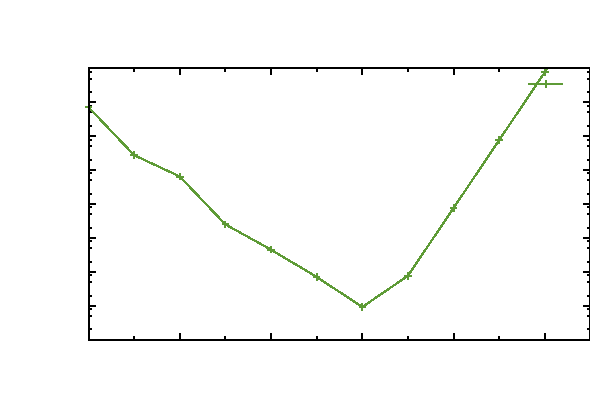
\includegraphics{fdvalidation}}%
%   Scaled-down include
    \put(0,0){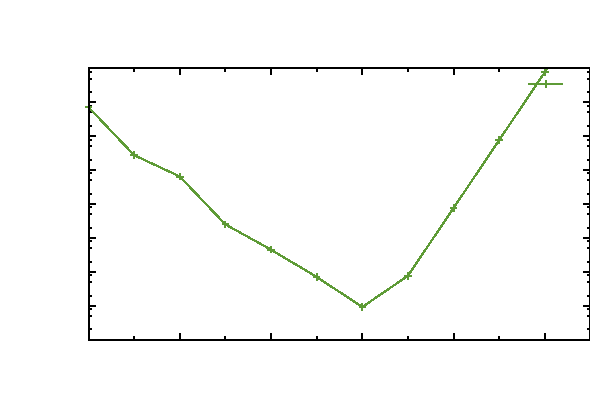
\includegraphics[scale=.5]{fdvalidation}}%
    \gplfronttext
  \end{picture}%
\endgroup
}}
    \only<2>{\centerline{% GNUPLOT: LaTeX picture with Postscript
\begingroup
  \makeatletter
  \providecommand\color[2][]{%
    \GenericError{(gnuplot) \space\space\space\@spaces}{%
      Package color not loaded in conjunction with
      terminal option `colourtext'%
    }{See the gnuplot documentation for explanation.%
    }{Either use 'blacktext' in gnuplot or load the package
      color.sty in LaTeX.}%
    \renewcommand\color[2][]{}%
  }%
  \providecommand\includegraphics[2][]{%
    \GenericError{(gnuplot) \space\space\space\@spaces}{%
      Package graphicx or graphics not loaded%
    }{See the gnuplot documentation for explanation.%
    }{The gnuplot epslatex terminal needs graphicx.sty or graphics.sty.}%
    \renewcommand\includegraphics[2][]{}%
  }%
  \providecommand\rotatebox[2]{#2}%
  \@ifundefined{ifGPcolor}{%
    \newif\ifGPcolor
    \GPcolortrue
  }{}%
  \@ifundefined{ifGPblacktext}{%
    \newif\ifGPblacktext
    \GPblacktextfalse
  }{}%
  % define a \g@addto@macro without @ in the name:
  \let\gplgaddtomacro\g@addto@macro
  % define empty templates for all commands taking text:
  \gdef\gplbacktext{}%
  \gdef\gplfronttext{}%
  \makeatother
  \ifGPblacktext
    % no textcolor at all
    \def\colorrgb#1{}%
    \def\colorgray#1{}%
  \else
    % gray or color?
    \ifGPcolor
      \def\colorrgb#1{\color[rgb]{#1}}%
      \def\colorgray#1{\color[gray]{#1}}%
      \expandafter\def\csname LTw\endcsname{\color{white}}%
      \expandafter\def\csname LTb\endcsname{\color{black}}%
      \expandafter\def\csname LTa\endcsname{\color{black}}%
      \expandafter\def\csname LT0\endcsname{\color[rgb]{1,0,0}}%
      \expandafter\def\csname LT1\endcsname{\color[rgb]{0,1,0}}%
      \expandafter\def\csname LT2\endcsname{\color[rgb]{0,0,1}}%
      \expandafter\def\csname LT3\endcsname{\color[rgb]{1,0,1}}%
      \expandafter\def\csname LT4\endcsname{\color[rgb]{0,1,1}}%
      \expandafter\def\csname LT5\endcsname{\color[rgb]{1,1,0}}%
      \expandafter\def\csname LT6\endcsname{\color[rgb]{0,0,0}}%
      \expandafter\def\csname LT7\endcsname{\color[rgb]{1,0.3,0}}%
      \expandafter\def\csname LT8\endcsname{\color[rgb]{0.5,0.5,0.5}}%
    \else
      % gray
      \def\colorrgb#1{\color{black}}%
      \def\colorgray#1{\color[gray]{#1}}%
      \expandafter\def\csname LTw\endcsname{\color{white}}%
      \expandafter\def\csname LTb\endcsname{\color{black}}%
      \expandafter\def\csname LTa\endcsname{\color{black}}%
      \expandafter\def\csname LT0\endcsname{\color{black}}%
      \expandafter\def\csname LT1\endcsname{\color{black}}%
      \expandafter\def\csname LT2\endcsname{\color{black}}%
      \expandafter\def\csname LT3\endcsname{\color{black}}%
      \expandafter\def\csname LT4\endcsname{\color{black}}%
      \expandafter\def\csname LT5\endcsname{\color{black}}%
      \expandafter\def\csname LT6\endcsname{\color{black}}%
      \expandafter\def\csname LT7\endcsname{\color{black}}%
      \expandafter\def\csname LT8\endcsname{\color{black}}%
    \fi
  \fi
%  Original size:
%  \setlength{\unitlength}{0.0500bp}%
% Half the original size
  \setlength{\unitlength}{0.0250bp}%
  \begin{picture}(5668.00,3968.00)%
    \gplgaddtomacro\gplbacktext{%
      \csname LTb\endcsname%
      \put(718,704){\makebox(0,0)[r]{\strut{}\scriptsize $10^{-10}$}}%
      \put(718,1030){\makebox(0,0)[r]{\strut{}\scriptsize $10^{-9}$}}%
      \put(718,1355){\makebox(0,0)[r]{\strut{}\scriptsize $10^{-8}$}}%
      \put(718,1681){\makebox(0,0)[r]{\strut{}\scriptsize $10^{-7}$}}%
      \put(718,2006){\makebox(0,0)[r]{\strut{}\scriptsize $10^{-6}$}}%
      \put(718,2332){\makebox(0,0)[r]{\strut{}\scriptsize $10^{-5}$}}%
      \put(718,2657){\makebox(0,0)[r]{\strut{}\scriptsize $10^{-4}$}}%
      \put(718,2983){\makebox(0,0)[r]{\strut{}\scriptsize $10^{-3}$}}%
      \put(718,3308){\makebox(0,0)[r]{\strut{}\scriptsize $10^{-2}$}}%
      \put(850,484){\makebox(0,0){\strut{}\scriptsize $10^{-12}$}}%
      \put(1726,484){\makebox(0,0){\strut{}\scriptsize $10^{-10}$}}%
      \put(2602,484){\makebox(0,0){\strut{}\scriptsize $10^{-8}$}}%
      \put(3478,484){\makebox(0,0){\strut{}\scriptsize $10^{-6}$}}%
      \put(4354,484){\makebox(0,0){\strut{}\scriptsize $10^{-4}$}}%
      \put(5230,484){\makebox(0,0){\strut{}\scriptsize $10^{-2}$}}%
      \put(80,2006){\rotatebox{90}{\makebox(0,0){\strut{}error}}}%
      \put(3259,154){\makebox(0,0){\strut{}Finite difference perturbation}}%
      \put(3259,3638){\makebox(0,0){\strut{}Validation of adjoint gradient wrt. finite differences}}%
    }%
    \gplgaddtomacro\gplfronttext{%
      \csname LTb\endcsname%
      \put(4945,3157){\makebox(0,0)[r]{\strut{}\scriptsize $\Vert\nabla_{FD}-\nabla_{adj}\Vert_2$}}%
    }%
    \gplbacktext
%   Original include, unscaled.
%    \put(0,0){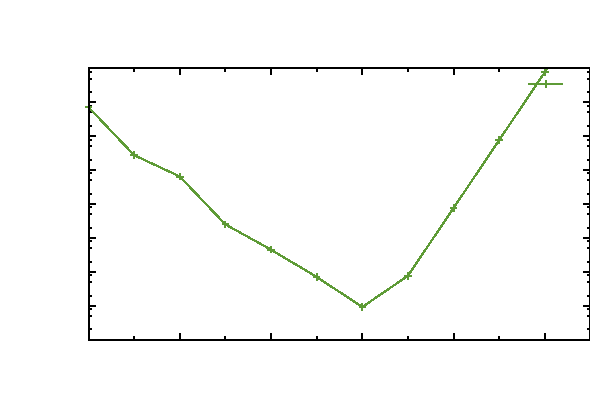
\includegraphics{fdvalidation}}%
%   Scaled-down include
    \put(0,0){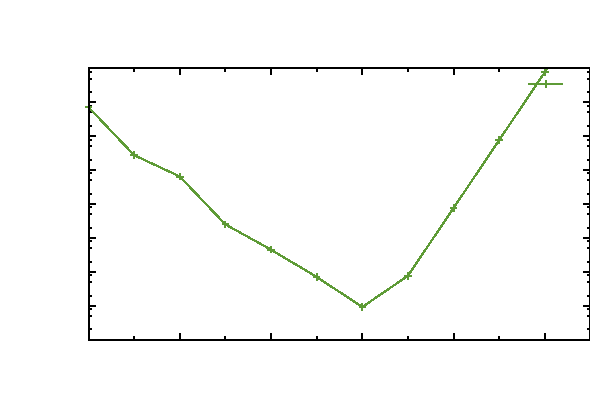
\includegraphics[scale=.5]{fdvalidation}}%
    \gplfronttext
  \end{picture}%
\endgroup
}}
    \only<3>{\centerline{% GNUPLOT: LaTeX picture with Postscript
\begingroup
  \makeatletter
  \providecommand\color[2][]{%
    \GenericError{(gnuplot) \space\space\space\@spaces}{%
      Package color not loaded in conjunction with
      terminal option `colourtext'%
    }{See the gnuplot documentation for explanation.%
    }{Either use 'blacktext' in gnuplot or load the package
      color.sty in LaTeX.}%
    \renewcommand\color[2][]{}%
  }%
  \providecommand\includegraphics[2][]{%
    \GenericError{(gnuplot) \space\space\space\@spaces}{%
      Package graphicx or graphics not loaded%
    }{See the gnuplot documentation for explanation.%
    }{The gnuplot epslatex terminal needs graphicx.sty or graphics.sty.}%
    \renewcommand\includegraphics[2][]{}%
  }%
  \providecommand\rotatebox[2]{#2}%
  \@ifundefined{ifGPcolor}{%
    \newif\ifGPcolor
    \GPcolortrue
  }{}%
  \@ifundefined{ifGPblacktext}{%
    \newif\ifGPblacktext
    \GPblacktextfalse
  }{}%
  % define a \g@addto@macro without @ in the name:
  \let\gplgaddtomacro\g@addto@macro
  % define empty templates for all commands taking text:
  \gdef\gplbacktext{}%
  \gdef\gplfronttext{}%
  \makeatother
  \ifGPblacktext
    % no textcolor at all
    \def\colorrgb#1{}%
    \def\colorgray#1{}%
  \else
    % gray or color?
    \ifGPcolor
      \def\colorrgb#1{\color[rgb]{#1}}%
      \def\colorgray#1{\color[gray]{#1}}%
      \expandafter\def\csname LTw\endcsname{\color{white}}%
      \expandafter\def\csname LTb\endcsname{\color{black}}%
      \expandafter\def\csname LTa\endcsname{\color{black}}%
      \expandafter\def\csname LT0\endcsname{\color[rgb]{1,0,0}}%
      \expandafter\def\csname LT1\endcsname{\color[rgb]{0,1,0}}%
      \expandafter\def\csname LT2\endcsname{\color[rgb]{0,0,1}}%
      \expandafter\def\csname LT3\endcsname{\color[rgb]{1,0,1}}%
      \expandafter\def\csname LT4\endcsname{\color[rgb]{0,1,1}}%
      \expandafter\def\csname LT5\endcsname{\color[rgb]{1,1,0}}%
      \expandafter\def\csname LT6\endcsname{\color[rgb]{0,0,0}}%
      \expandafter\def\csname LT7\endcsname{\color[rgb]{1,0.3,0}}%
      \expandafter\def\csname LT8\endcsname{\color[rgb]{0.5,0.5,0.5}}%
    \else
      % gray
      \def\colorrgb#1{\color{black}}%
      \def\colorgray#1{\color[gray]{#1}}%
      \expandafter\def\csname LTw\endcsname{\color{white}}%
      \expandafter\def\csname LTb\endcsname{\color{black}}%
      \expandafter\def\csname LTa\endcsname{\color{black}}%
      \expandafter\def\csname LT0\endcsname{\color{black}}%
      \expandafter\def\csname LT1\endcsname{\color{black}}%
      \expandafter\def\csname LT2\endcsname{\color{black}}%
      \expandafter\def\csname LT3\endcsname{\color{black}}%
      \expandafter\def\csname LT4\endcsname{\color{black}}%
      \expandafter\def\csname LT5\endcsname{\color{black}}%
      \expandafter\def\csname LT6\endcsname{\color{black}}%
      \expandafter\def\csname LT7\endcsname{\color{black}}%
      \expandafter\def\csname LT8\endcsname{\color{black}}%
    \fi
  \fi
%  Original size:
%  \setlength{\unitlength}{0.0500bp}%
% Half the original size
  \setlength{\unitlength}{0.0250bp}%
  \begin{picture}(5668.00,3968.00)%
    \gplgaddtomacro\gplbacktext{%
      \csname LTb\endcsname%
      \put(718,704){\makebox(0,0)[r]{\strut{}\scriptsize $10^{-10}$}}%
      \put(718,1030){\makebox(0,0)[r]{\strut{}\scriptsize $10^{-9}$}}%
      \put(718,1355){\makebox(0,0)[r]{\strut{}\scriptsize $10^{-8}$}}%
      \put(718,1681){\makebox(0,0)[r]{\strut{}\scriptsize $10^{-7}$}}%
      \put(718,2006){\makebox(0,0)[r]{\strut{}\scriptsize $10^{-6}$}}%
      \put(718,2332){\makebox(0,0)[r]{\strut{}\scriptsize $10^{-5}$}}%
      \put(718,2657){\makebox(0,0)[r]{\strut{}\scriptsize $10^{-4}$}}%
      \put(718,2983){\makebox(0,0)[r]{\strut{}\scriptsize $10^{-3}$}}%
      \put(718,3308){\makebox(0,0)[r]{\strut{}\scriptsize $10^{-2}$}}%
      \put(850,484){\makebox(0,0){\strut{}\scriptsize $10^{-12}$}}%
      \put(1726,484){\makebox(0,0){\strut{}\scriptsize $10^{-10}$}}%
      \put(2602,484){\makebox(0,0){\strut{}\scriptsize $10^{-8}$}}%
      \put(3478,484){\makebox(0,0){\strut{}\scriptsize $10^{-6}$}}%
      \put(4354,484){\makebox(0,0){\strut{}\scriptsize $10^{-4}$}}%
      \put(5230,484){\makebox(0,0){\strut{}\scriptsize $10^{-2}$}}%
      \put(80,2006){\rotatebox{90}{\makebox(0,0){\strut{}error}}}%
      \put(3259,154){\makebox(0,0){\strut{}Finite difference perturbation}}%
      \put(3259,3638){\makebox(0,0){\strut{}Validation of adjoint gradient wrt. finite differences}}%
    }%
    \gplgaddtomacro\gplfronttext{%
      \csname LTb\endcsname%
      \put(4945,3157){\makebox(0,0)[r]{\strut{}\scriptsize $\Vert\nabla_{FD}-\nabla_{adj}\Vert_2$}}%
    }%
    \gplbacktext
%   Original include, unscaled.
%    \put(0,0){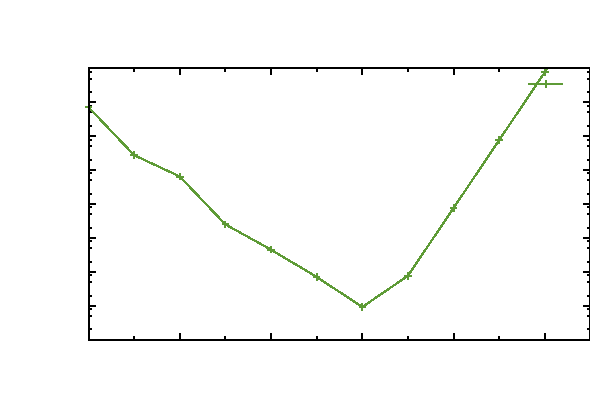
\includegraphics{fdvalidation}}%
%   Scaled-down include
%    \put(0,0){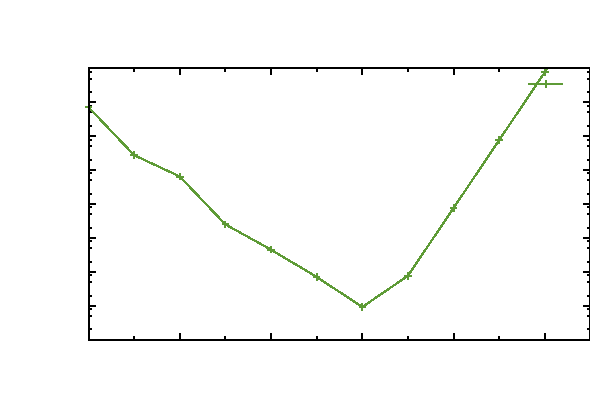
\includegraphics[scale=.5]{fdvalidation}}%
    \gplfronttext
  \end{picture}%
\endgroup
}}
  \end{overlayarea}

  \only<1>{\centerline{The graph only}}
  \only<2>{\centerline{Graph and Text}}
  \only<3>{\centerline{Text only}}
\end{frame}

\section[Animation]{``You gotta move it, move it!''}

\begin{frame}{Films}
  None of the Linux-based viewers allow you to embed a video, but
  you can launch your player with a click on the still image:

  \begin{columns}
    \begin{column}<+->{.4\textwidth}
      \movie[externalviewer]
      {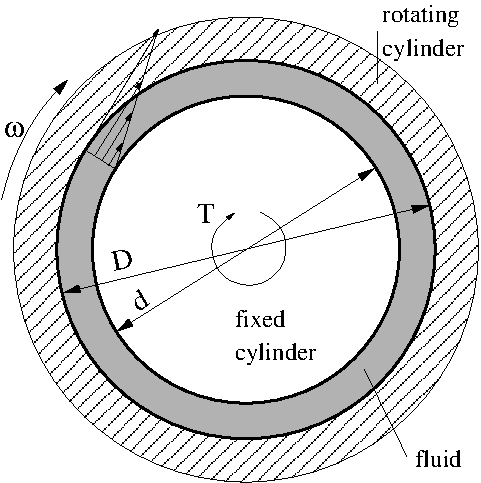
\includegraphics[width=\textwidth]{concentric_cylinder}}
      {figures/Glyzerin.mpg}
    \end{column}
    \begin{column}{.59\textwidth}
      \begin{itemize}
      \item You will need to install and add the {\tt multimedia}
      latex package.
        
      \item The player will not understand the \ltx{graphicspath}
      command, you need to explicitly give the path to the film.
    \item Mac and Windows pdf readers may be able to use embedded
      movies.
      \end{itemize}
    \end{column}
  \end{columns}

\end{frame}

\begin{frame}{Animations}
  For most of our shape optimisation work we only want to 
  show a few iterations, this is nicely done using {\tt animations}:

\centerline{
  % Find the manual at
  % http://ctan.math.utah.edu/ctan/tex-archive/macros/latex/contrib/animate/animate.pdf
  \animategraphics[loop,width=.5\textwidth]{6}
    {./figures/animations/LaplacianSmoothing/smoothingEx-}{1}{20}
  }
  You will need to include the {\tt animate} package.
  The Linux pdf reader evince won't understand this, but 
  Adobe's acroread does.  

  \slidefoot{Contributed by: Shenren, Mateusz}

\end{frame}

\section[Code]{A few ways of showing code}


\begin{frame}{Code example with columns and uncovering} 

  \begin{equation*}
    \mathbf{y} = 
  \left[
    \begin{array}{c}
      y_1 \\ y_2
    \end{array}
  \right]
  =
  \left[\begin{array}{l}
 \pi\cdot\cos(3x_1+2x_2+x_3)\cdot\pi\cdot\sin(3x_1+2x_2+x_3)\\   
 \pi\cdot\sin(3x_1+2x_2+x_3)\cdot x_1\\   
  \end{array}\right]
  \end{equation*}

  \vfill
  \begin{columns}
    \begin{column}<2->{.49\textwidth}
      {\small\tt
        u = 3*x(1)+2*x(2)+x(3) \\
        pi = 3.14 \\
        v = pi*cos(u) \\
        w = pi*sin(u) \\
        sum = v + u \\
        y(1) = v * w \\
        y(2) = w*x(1) \\
      }
    \end{column}
%
    \begin{column}{.49\textwidth}
      {\small\tt
        \uncover<6->{%
          gx(1) = 1\\ 
          gx(2) = gx(3) = 0\\
        }
        \uncover<5->{
          gu = 3*gx(1)+2*gx(2)+gx(3)\\}
        \uncover<4->{
          gv = -pi*sin(u)*gu\\
          gw = pi*cos(u)*gu\\
          gy(1) = gv*w + v*gw\\}
        \uncover<3->{        
          gy(2) = gw*x(1) + gx(1)*w\\}
      }
    \end{column}
  \end{columns}

%\source{Kaminski, Giering, 2002}, JDM added y(2)
\end{frame}


\begin{frame}{A simple example}
Full size font, indents controlled with \ltx{hspace} and variable
width.

\vfill
DO iter=1,n {\color{green}!Nonlinear iteration}\\
\hspace{0.6cm}DO istep=1,nstep{\color{green}!Runge-Kutta}\\
\hspace{1.2cm}IF(istep .EQ. 1) then\\
\hspace{1.8cm}		CALL {\color{blue}calc\_timestep}\\
\hspace{1.8cm}		CALL {\color{blue}calc\_jacob}\\
\hspace{1cm}\\
\hspace{1.2cm}    ENDIF	\\
\hspace{1.2cm}   CALL {\color{blue}calc\_res}\\
\hspace{1.2cm}   CALL {\color{blue}update}{\color{green}!SGS} \\
\hspace{0.6cm}ENDDO\\
\hspace{0.6cm}CALL {\color{blue}MG\_restriction/prolongation} {\color{green}!Multigrid}\\
\hspace{0.0cm}ENDDO

\end{frame}


\newcommand{\indt}{\hspace{.05\textwidth}}
\newcommand{\indth}{\hspace{.029\textwidth}}

\begin{frame}{A macro for the fixed space reduces typing}
  This example here uses a spacing macro \ltx{indt} to 
  create fixed indents (use it twice for double indentation). 
  
  And using a \ltx{small} font size.

  \vfill
  {\small 
    \uncover<2->{set $k=1$, $x_k = x_{start}$ \\} 
    \uncover<3->{\textbf{do}\\} 
    \uncover<4->{\indt compute $F(x_k)$, $\nabla F(x_k)$ \\} 
    \uncover<5->{\indt set $p_k = -\nabla F(x_k)$\\}
    \uncover<6->{\indt find $s$ to minimise $\varphi(s) = F(x_k\!+\!s p_k)$
          ! line search\\}
    \uncover<7->{\indt set $x_{k+1} = x_k + s p_k$\\}
    \uncover<3->{\textbf{while} $||\nabla F(x_k)|| \geq \varepsilon$ }
  }
\end{frame}


\begin{frame}[fragile]{A better example, using lslisting}
\begin{lstlisting}[gobble=2, language=Fortran]
  DO iter=1,n ! Nonlinear iteration
    DO istep=1,nstep ! Runge-Kutta
      IF(istep .EQ. 1) then
        CALL calc_timestep
        CALL calc_jacob
      ENDIF
      CALL calc_res
      CALL update !SGS
    ENDDO
    CALL MG_restriction/prolongation ! Multigrid
  ENDDO
\end{lstlisting}

\slidefoot{Proposed by: Jan}


\end{frame}

\begin{frame}[fragile]{How to input source code more easily}
Copy and paste this into your header:
\lstinputlisting[language=TeX, firstline=13, lastline=19]{talk.tex}
\end{frame}
\begin{frame}[fragile]{How to input source code more easily, cont'd}
Code can also be included from a file (ex.f90):
\lstinputlisting[language=Fortran, firstline=5, lastline=15]{ex.f90}
\end{frame}



\section{Summary}

\begin{frame}{Summary}

 
  It might be {\tt foo}

  \vfill
  But then Laurent says it is {\tt foo\_bar}

  \vfill
  \uncover<2->{
  We have now shown that it is simply \uncover<3->{\tt blah}}, 
  \uncover<4->{or actually {\tt diblah} and then {\tt obladibladah}}.
\end{frame}
